\documentclass[11pt,aspectratio=169]{beamer}

\usepackage[utf8]{inputenc}
\usepackage[T1]{fontenc}
\usepackage{helvet}
\usepackage{amsmath, amssymb, bm}
\usepackage{booktabs}
\usepackage{array}
\usepackage{tikz}
\usetikzlibrary{arrows.meta, positioning, calc}
\usepackage{hyperref}

% ------------------------------------------------------------------
% Basic Beamer template with a simple color accent
% ------------------------------------------------------------------
\usetheme{default}
\usefonttheme[onlymath]{serif}
\setbeamertemplate{navigation symbols}{}
\setbeamertemplate{itemize items}[circle]
\setbeamertemplate{enumerate items}[default]
\setbeamertemplate{bibliography item}[text]

\definecolor{Main}{RGB}{25, 70, 140}
\definecolor{Accent}{RGB}{0, 120, 128}
\definecolor{Warn}{RGB}{185, 45, 45}
\definecolor{Soft}{RGB}{236, 242, 250}

\setbeamercolor{structure}{fg=Main}
\setbeamercolor{frametitle}{fg=Main}
\setbeamercolor{title}{fg=Main}
\setbeamercolor{subtitle}{fg=Accent}
\setbeamerfont{frametitle}{size=\Large,series=\bfseries}
\setbeamerfont{title}{size=\LARGE,series=\bfseries}

\setbeamertemplate{frametitle}{%
  \vspace{0.3cm}\insertframetitle\par\vspace{0.08cm}%
  {\color{Main!60}\hrule height 0.8pt}\vspace{0.05cm}}
\setbeamertemplate{footline}{%
  \hfill\footnotesize\textcolor{Main!70}{\insertframenumber\,/\,\inserttotalframenumber}\hspace{0.45cm}\vspace{0.2cm}}

\setbeamersize{text margin left=0.8cm, text margin right=0.8cm}
\setlength{\leftmargini}{1.1em}

\newcommand{\Head}[1]{\textcolor{Main}{\textbf{#1}}}
\newcommand{\Key}[1]{\textcolor{Accent}{\textbf{#1}}}

% Figure helper: works whether compiled from repo root or report/
\newcommand{\Fig}[2]{%
  \IfFileExists{../experiments/figures/#1}%
    {\includegraphics[#2]{../experiments/figures/#1}}%
    {\IfFileExists{experiments/figures/#1}%
      {\includegraphics[#2]{experiments/figures/#1}}%
      {\fbox{\scriptsize missing: #1}}}}

\title{Diffusion Models: From Adding Noise to Generating Images}
\subtitle{CS420 Seminar [S06]}
\author{Vong Chi Van (24125049) \quad Le Dat Phuc An (24125052)}
\institute{University of Science, VNU-HCM\\[2pt]
  \footnotesize\url{https://github.com/ChiVan222/AI_Seminar_Diffusion}}
\date{}

\begin{document}

% ==================================================================
\begin{frame}
  \titlepage
  \vspace{-0.6cm}
  \begin{center}
    \footnotesize\color{black!70}
    Part I (Slides 2--6): Vong Chi Van \qquad Part II (Slides 7--11): Le Dat Phuc An
  \end{center}
\end{frame}

% ==================================================================
\begin{frame}{Problem \& Guiding Question}
  \Head{Goal of generative modeling:} learn the data distribution $p(\mathbf{x})$ so we can sample \emph{new} images.

  \vspace{0.15cm}
  \Head{Earlier approaches each give something up:}
  \begin{itemize}
    \item \textbf{VAEs} are fast, but samples are blurry.
    \item \textbf{GANs} are sharp, but training is unstable and they miss modes.
    \item \textbf{Autoregressive models} are exact, but generate one pixel at a time.
  \end{itemize}

  \vspace{0.15cm}
  \begin{center}
    \colorbox{Soft}{\parbox{0.9\textwidth}{\centering\vspace{3pt}
      \textit{How can learning to remove noise step by step let a network generate images, and why does moving this process into a latent space make it much cheaper?}\vspace{3pt}}}
  \end{center}

  \vspace{0.05cm}
  \small
  \textbf{Papers:} DDPM, Ho et al., NeurIPS 2020 \cite{ho2020denoising} (required) \;$\cdot$\;
  Latent Diffusion, Rombach et al., CVPR 2022 \cite{rombach2022high}\\
  \textbf{Our experiments:} re-implemented on MNIST, trained on one NVIDIA T4 GPU.
\end{frame}

% ==================================================================
\begin{frame}{Task 1 --- Discriminative vs.\ Generative Models}
  \begin{columns}[T,onlytextwidth]
    \begin{column}{0.45\textwidth}
      \begin{itemize}
        \item \textbf{Discriminative} $P(y\mid\mathbf{x})$: learns a \emph{boundary} between classes. It classifies, but it cannot create data.
        \item \textbf{Generative} $p(\mathbf{x})$: learns \emph{where data lives}, so it can sample new $\mathbf{x}$.
      \end{itemize}
      \vspace{0.15cm}
      \centering
      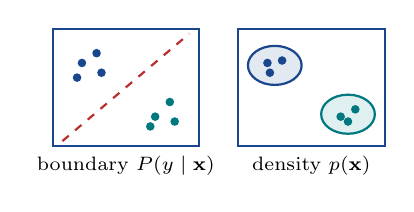
\begin{tikzpicture}[scale=0.62]
        \draw[Main, thick] (0,0) rectangle (3,2.4);
        \draw[Warn, thick, dashed] (0.2,0.1) -- (2.8,2.3);
        \foreach \p in {(0.6,1.7),(0.9,1.9),(0.5,1.4),(1.0,1.5)} \fill[Main] \p circle (2.5pt);
        \foreach \p in {(2.1,0.6),(2.4,0.9),(2.0,0.4),(2.5,0.5)} \fill[Accent] \p circle (2.5pt);
        \node[below, font=\scriptsize] at (1.5,0) {boundary $P(y\mid\mathbf{x})$};
        \begin{scope}[xshift=3.8cm]
          \draw[Main, thick] (0,0) rectangle (3,2.4);
          \draw[Main, thick, fill=Main!12] (0.75,1.65) ellipse (0.55 and 0.4);
          \draw[Accent, thick, fill=Accent!12] (2.25,0.65) ellipse (0.55 and 0.4);
          \foreach \p in {(0.6,1.7),(0.9,1.75),(0.65,1.5)} \fill[Main] \p circle (2.5pt);
          \foreach \p in {(2.1,0.6),(2.4,0.75),(2.25,0.5)} \fill[Accent] \p circle (2.5pt);
          \node[below, font=\scriptsize] at (1.5,0) {density $p(\mathbf{x})$};
        \end{scope}
      \end{tikzpicture}
    \end{column}
    \begin{column}{0.52\textwidth}
      \Head{Qualitative comparison}
      \vspace{0.1cm}

      \small
      \setlength{\tabcolsep}{4pt}
      \renewcommand{\arraystretch}{1.3}
      \begin{tabular}{@{}lccc@{}}
        \toprule
        & \textbf{Quality} & \textbf{Diversity} & \textbf{Speed} \\
        \midrule
        VAE \cite{kingma2014auto}            & {\color{Warn}blurry} & good & {\color{Accent}fast} \\
        GAN \cite{goodfellow2014generative}  & {\color{Accent}sharp} & {\color{Warn}collapse} & {\color{Accent}fast} \\
        PixelCNN \cite{oord2016pixel}        & sharp & good & {\color{Warn}very slow} \\
        \textbf{Diffusion} \cite{ho2020denoising} & {\color{Accent}\textbf{sharp}} & {\color{Accent}\textbf{good}} & {\color{Warn}slow} \\
        \bottomrule
      \end{tabular}

      \vspace{0.3cm}
      \normalsize
      Diffusion gives up \emph{speed} to get both quality and diversity. LDM is designed to recover that speed.
    \end{column}
  \end{columns}
\end{frame}

% ==================================================================
\begin{frame}{Task 2 --- Forward Noising and Reverse Denoising}
  \centering
  \resizebox{0.95\textwidth}{!}{%
  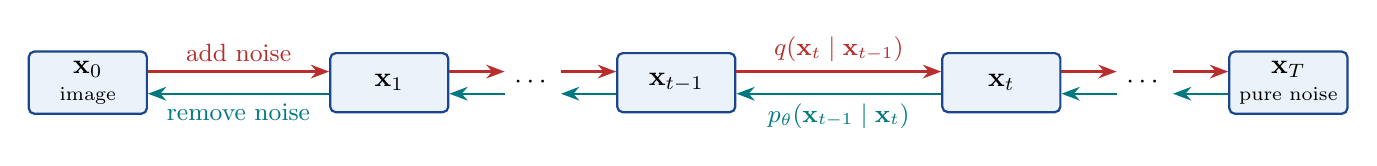
\begin{tikzpicture}[
      st/.style={draw=Main, fill=Soft, thick, rounded corners=2pt, minimum width=1.5cm, minimum height=0.75cm, align=center},
      fwd/.style={-{Stealth}, thick, Warn},
      rev/.style={-{Stealth}, thick, Accent}]
    \node[st] (x0) {$\mathbf{x}_0$\\[-2pt]\scriptsize image};
    \node[st, right=2.3cm of x0] (x1) {$\mathbf{x}_1$};
    \node[right=0.7cm of x1] (d1) {$\cdots$};
    \node[st, right=0.7cm of d1] (xtm) {$\mathbf{x}_{t-1}$};
    \node[st, right=2.6cm of xtm] (xt) {$\mathbf{x}_t$};
    \node[right=0.7cm of xt] (d2) {$\cdots$};
    \node[st, right=0.7cm of d2] (xT) {$\mathbf{x}_T$\\[-2pt]\scriptsize pure noise};
    \foreach \a/\b in {x0/x1, x1/d1, d1/xtm, xtm/xt, xt/d2, d2/xT}{
      \draw[fwd] ([yshift=4pt]\a.east) -- ([yshift=4pt]\b.west);
      \draw[rev] ([yshift=-4pt]\b.west) -- ([yshift=-4pt]\a.east);}
    \node[above=4pt, Warn, font=\small] at ($(xtm.east)!0.5!(xt.west)$) {$q(\mathbf{x}_t\mid\mathbf{x}_{t-1})$};
    \node[below=4pt, Accent, font=\small] at ($(xtm.east)!0.5!(xt.west)$) {$p_\theta(\mathbf{x}_{t-1}\mid\mathbf{x}_t)$};
    \node[above=4pt, Warn, font=\small] at ($(x0.east)!0.5!(x1.west)$) {add noise};
    \node[below=4pt, Accent, font=\small] at ($(x0.east)!0.5!(x1.west)$) {remove noise};
  \end{tikzpicture}}

  \vspace{0.2cm}
  \begin{columns}[T,onlytextwidth]
    \begin{column}{0.48\textwidth}
      \Head{Forward process (fixed, no learning)}
      \[ q(\mathbf{x}_t\mid\mathbf{x}_{t-1}) = \mathcal{N}\big(\sqrt{1-\beta_t}\,\mathbf{x}_{t-1},\ \beta_t\mathbf{I}\big) \]
      \small Small noise $\beta_t\in(0,1)$ is added at each step. Any step can be reached directly:
      \[ \mathbf{x}_t = \sqrt{\bar\alpha_t}\,\mathbf{x}_0 + \sqrt{1-\bar\alpha_t}\,\bm\epsilon,\quad \bar\alpha_t=\textstyle\prod_{s\le t}(1-\beta_s) \]
    \end{column}
    \begin{column}{0.48\textwidth}
      \Head{Reverse process (learned)}
      \begin{itemize}\small
        \item A U-Net $\bm\epsilon_\theta(\mathbf{x}_t,t)$ predicts the noise $\bm\epsilon$ that was added.
        \item Training objective \cite{ho2020denoising}:
      \end{itemize}
      \[ L_{\text{simple}} = \mathbb{E}_{t,\mathbf{x}_0,\bm\epsilon}\big\|\bm\epsilon-\bm\epsilon_\theta(\mathbf{x}_t,t)\big\|^2 \]
      \small Equivalent to learning the score $\nabla_{\mathbf{x}}\log p(\mathbf{x})$ \cite{song2019generative}.
    \end{column}
  \end{columns}
\end{frame}

% ==================================================================
\begin{frame}{Task 2 --- Training and Sampling Algorithms}
  \begin{columns}[T,onlytextwidth]
    \begin{column}{0.47\textwidth}
      \Head{Algorithm 1: Training}
      \vspace{0.1cm}
      \begin{enumerate}
        \item Take a real image $\mathbf{x}_0$
        \item Pick a random step $t\in\{1,\dots,T\}$ and noise $\bm\epsilon\sim\mathcal{N}(\mathbf{0},\mathbf{I})$
        \item Make $\mathbf{x}_t=\sqrt{\bar\alpha_t}\mathbf{x}_0+\sqrt{1-\bar\alpha_t}\bm\epsilon$
        \item Update $\theta$ to minimize $\|\bm\epsilon-\bm\epsilon_\theta(\mathbf{x}_t,t)\|^2$
      \end{enumerate}
      \vspace{0.15cm}
      \small\color{black!75}
      Each step is a simple regression with \textbf{one} network pass, so training is stable.
    \end{column}
    \begin{column}{0.49\textwidth}
      \Head{Algorithm 2: Sampling}
      \vspace{0.1cm}
      \begin{enumerate}
        \item Start from pure noise $\mathbf{x}_T\sim\mathcal{N}(\mathbf{0},\mathbf{I})$
        \item For $t=T,\dots,1$, remove the predicted noise:
      \end{enumerate}
      \[ \mathbf{x}_{t-1}=\tfrac{1}{\sqrt{\alpha_t}}\Big(\mathbf{x}_t-\tfrac{\beta_t}{\sqrt{1-\bar\alpha_t}}\bm\epsilon_\theta(\mathbf{x}_t,t)\Big)+\sigma_t\mathbf{z} \]
      \begin{enumerate}\setcounter{enumi}{2}
        \item Return $\mathbf{x}_0$
      \end{enumerate}
      \vspace{0.05cm}
      \small\color{black!75}
      Needs $T$ \textbf{sequential} network passes ($T=1000$ in \cite{ho2020denoising}). This is why sampling is slow.
    \end{column}
  \end{columns}
\end{frame}

% ==================================================================
\begin{frame}{Task 3 --- A 1D Worked Example}
  \begin{columns}[T,onlytextwidth]
    \begin{column}{0.4\textwidth}
      \Head{Symbols}
      \vspace{0.1cm}

      \small
      \renewcommand{\arraystretch}{1.25}
      \begin{tabular}{@{}cl@{}}
        \toprule
        $\mathbf{x}_0$ & clean data, scaled to $[-1,1]$ \\
        $\mathbf{x}_t$ & noisy data at step $t$ \\
        $\beta_t$ & noise variance, $(0,1)$ \\
        $\bar\alpha_t$ & signal kept, from $1$ to $0$ \\
        $\bm\epsilon$ & Gaussian noise $\mathcal{N}(\mathbf{0},\mathbf{I})$ \\
        $\bm\epsilon_\theta$ & network's noise guess \\
        \bottomrule
      \end{tabular}

      \vspace{0.25cm}
      \textbf{Given:} $x_0=0.80$, $\beta_1=0.19$, $\epsilon=-0.50$\\
      $\Rightarrow\ \sqrt{\bar\alpha_1}=0.90,\ \sqrt{1-\bar\alpha_1}=0.436$
    \end{column}
    \begin{column}{0.56\textwidth}
      \Head{1.\ Forward step}
      \[ x_1 = 0.90(0.80) + 0.436(-0.50) = \mathbf{0.502} \]
      \small The mean shrinks toward 0 ($0.72$) while noise is added, which keeps the total variance at 1.

      \vspace{0.15cm}
      \normalsize\Head{2.\ Loss} \small (suppose the network predicts $\epsilon_\theta=-0.30$)
      \[ L = (-0.50 - (-0.30))^2 = \mathbf{0.04} \]

      \normalsize\Head{3.\ Reverse step}
      \[ \hat{x}_0 = \tfrac{1}{0.90}\big(0.502 + 0.436\times0.30\big) = \mathbf{0.703} \]
      \small With a perfect guess ($\epsilon_\theta=-0.50$) we recover exactly $\hat{x}_0=0.80$.
    \end{column}
  \end{columns}
\end{frame}

% ==================================================================
\begin{frame}{Tasks 1 \& 4 --- Experiments on MNIST}
  \begin{columns}[T,onlytextwidth]
    \begin{column}{0.5\textwidth}
      \Head{Same data, four model families}
      \vspace{0.1cm}

      \small
      \renewcommand{\arraystretch}{1.25}
      \begin{tabular}{@{}lrrr@{}}
        \toprule
        \textbf{Model} & \textbf{Steps} & \textbf{Time / 64} & \textbf{FID $\downarrow$} \\
        \midrule
        VAE       & 1   & 6.5 ms  & 82.3 \\
        PixelCNN  & 784 & 4.29 s  & 64.1 \\
        DCGAN     & 1   & 11.4 ms & 44.1 \\
        \textbf{DDPM} & 300 & 3.93 s & \Key{16.9} \\
        \bottomrule
      \end{tabular}

      \vspace{0.2cm}
      \footnotesize FID is computed with our MNIST classifier (98.85\% test accuracy).

      \vspace{0.2cm}
      \normalsize
      \begin{itemize}
        \item DDPM gives the \textbf{best quality}.
        \item It is about $\mathbf{350\times}$ \textbf{slower} than the GAN.
      \end{itemize}
    \end{column}
    \begin{column}{0.47\textwidth}
      \Head{Task 4: noising and denoising}
      \vspace{0.15cm}

      \centering
      \Fig{task1_and_4_diffusion_trajectories.png}{width=\linewidth,height=3.9cm,keepaspectratio}

      \vspace{0.1cm}
      \raggedright\small
      \textbf{Top:} the digit fades into noise.\\
      \textbf{Bottom:} a digit emerges from pure noise.
    \end{column}
  \end{columns}
\end{frame}

% ==================================================================
\begin{frame}{Task 5 --- Latent Diffusion Models \cite{rombach2022high}}
  \centering
  \resizebox{0.85\textwidth}{!}{%
  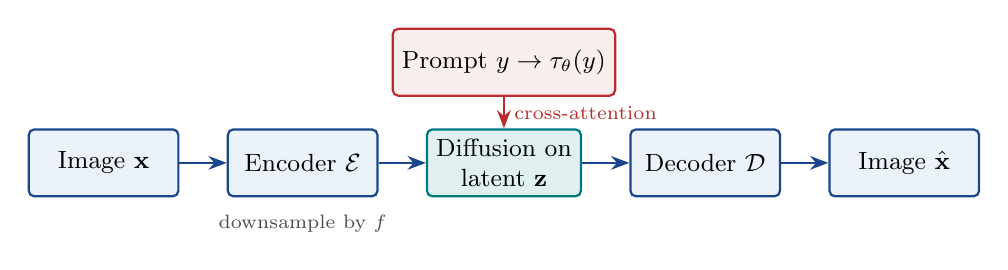
\begin{tikzpicture}[
      b/.style={draw=Main, fill=Soft, thick, rounded corners=2pt, minimum height=0.85cm, minimum width=1.9cm, align=center, font=\small},
      a/.style={-{Stealth}, thick, Main}]
    \node[b] (x) {Image $\mathbf{x}$};
    \node[b, right=0.6cm of x] (E) {Encoder $\mathcal{E}$};
    \node[b, right=0.6cm of E, fill=Accent!12, draw=Accent] (z) {Diffusion on\\latent $\mathbf{z}$};
    \node[b, right=0.6cm of z] (D) {Decoder $\mathcal{D}$};
    \node[b, right=0.6cm of D] (o) {Image $\hat{\mathbf{x}}$};
    \node[b, above=0.4cm of z, fill=Warn!8, draw=Warn] (y) {Prompt $y\to\tau_\theta(y)$};
    \draw[a] (x)--(E); \draw[a] (E)--(z); \draw[a] (z)--(D); \draw[a] (D)--(o);
    \draw[a, Warn] (y)--node[right, font=\scriptsize]{cross-attention}(z);
    \node[below=0.1cm of E, font=\scriptsize, black!70] {downsample by $f$};
  \end{tikzpicture}}

  \raggedright
  \begin{enumerate}\setlength{\itemsep}{1pt}
    \item \textbf{Compress:} an autoencoder maps the image to a small latent grid and discards fine pixel detail we cannot perceive.
    \item \textbf{Diffuse in latent space:} the same DDPM runs on $\mathbf{z}$. Attention cost drops by about $f^4$.
    \item \textbf{Condition:} prompt tokens act as keys/values in cross-attention,
      $\ \text{softmax}\!\big(\mathbf{Q}\mathbf{K}^\top/\sqrt{d}\big)\mathbf{V}$.
  \end{enumerate}
  \Head{Classifier-free guidance} (scale $\alpha$) pushes samples toward the prompt:
  \vspace{-0.15cm}
  \[ \tilde{\bm\epsilon} = \bm\epsilon_\theta(\mathbf{z}_t,\varnothing) + \alpha\,\big(\bm\epsilon_\theta(\mathbf{z}_t,y) - \bm\epsilon_\theta(\mathbf{z}_t,\varnothing)\big) \]
\end{frame}

% ==================================================================
\begin{frame}{Task 5 --- Our Latent Diffusion Results}
  \begin{columns}[T,onlytextwidth]
    \begin{column}{0.47\textwidth}
      \Head{Stage 1: VAE, $32{\times}32 \rightarrow 8{\times}8{\times}4$}
      \vspace{0.15cm}

      \centering
      \Fig{task5_vae_recon_strip.png}{width=\linewidth}

      \vspace{0.15cm}
      \raggedright
      \begin{itemize}
        \item Reconstruction \Key{FID 0.18}, PSNR 33.7 dB
        \item 99.8\% of digits keep their label
      \end{itemize}
      \small The small latent keeps almost all of the digit content.
    \end{column}
    \begin{column}{0.49\textwidth}
      \Head{Stage 2: prompt = digit label ``0''--``9''}
      \vspace{0.15cm}

      \small
      \renewcommand{\arraystretch}{1.3}
      \centering
      \begin{tabular}{@{}cccc@{}}
        \toprule
        \textbf{CFG $\alpha$} & \textbf{Prompt acc.} & \textbf{FID $\downarrow$} & \textbf{Saturated} \\
        \midrule
        1.0  & 94.0\%  & \Key{28.1} & 4.5\% \\
        3.0  & \Key{100\%} & 71.1 & 5.6\% \\
        7.5  & 99.5\% & 94.3 & 7.5\% \\
        15.0 & 99.5\% & 142.3 & {\color{Warn}10.6\%} \\
        \bottomrule
      \end{tabular}

      \vspace{0.25cm}
      \raggedright\normalsize
      \begin{itemize}
        \item Guidance makes the model \textbf{follow the prompt}.
        \item Too much guidance hurts \textbf{diversity} and causes \textbf{oversaturation}.
      \end{itemize}
    \end{column}
  \end{columns}
\end{frame}

% ==================================================================
\begin{frame}{Task 6 --- Pixel-Space vs.\ Latent-Space Diffusion}
  \small
  Same U-Net design, same data and training setup; only the space changes (T4 GPU).

  \vspace{0.1cm}
  \centering
  \small
  \renewcommand{\arraystretch}{1.25}
  \begin{tabular}{@{}p{3.3cm}p{4.6cm}p{4.6cm}@{}}
    \toprule
    & \textbf{Pixel diffusion (DDPM)} & \textbf{Latent diffusion (LDM)} \\
    \midrule
    Works on       & $32\times32\times1$ pixels & $8\times8\times4$ latent \\
    Training time  & 51.4 s / epoch & \Key{6.8 s / epoch \ ($7.6\times$)} \\
    Peak memory    & 1{,}152 MB & \Key{83 MB \ ($13.8\times$ less)} \\
    Quality        & strong at low resolution & strong at high resolution \cite{rombach2022high} \\
    Conditioning   & limited & flexible (cross-attention) \\
    Main weakness  & cost grows fast with size & capped by the autoencoder \\
    \bottomrule
  \end{tabular}

  \vspace{0.2cm}
  \raggedright
  \Head{Takeaway:} moving diffusion into a compressed latent space gives large compute savings with little loss in quality.
\end{frame}

% ==================================================================
\begin{frame}{Limitations \& Conclusion}
  \begin{columns}[T,onlytextwidth]
    \begin{column}{0.5\textwidth}
      \Head{Limitations}
      \begin{itemize}\setlength{\itemsep}{1pt}
        \item \textbf{Slow sampling:} many sequential steps. Faster samplers \cite{song2021denoising,lu2022dpm} help but lose some detail.
        \item \textbf{Prompt control:} strong guidance oversaturates; complex prompts are hard.
        \item \textbf{Memorization:} models can copy training images \cite{carlini2023extracting}.
        \item \textbf{Bias:} web-scale data carries social bias.
        \item \textbf{Our scope:} MNIST on one GPU. Gains should grow at high resolution, but we did not test that.
      \end{itemize}
    \end{column}
    \begin{column}{0.46\textwidth}
      \Head{Conclusion}
      \vspace{0.1cm}

      Diffusion models turn generation into a sequence of easy denoising steps. This gives sharp \emph{and} diverse samples with stable training.

      \vspace{0.2cm}
      Latent diffusion keeps these benefits but runs in a compact latent space. That makes high-resolution, prompt-controlled generation practical.
    \end{column}
  \end{columns}
\end{frame}

% ==================================================================
\begin{frame}{References \& Q\&A}
  \begin{columns}[T,onlytextwidth]
    \begin{column}{0.64\textwidth}
      \scriptsize
      \begin{thebibliography}{9}\setlength{\itemsep}{0pt}
        \bibitem{ho2020denoising} J.\ Ho, A.\ Jain, P.\ Abbeel. Denoising Diffusion Probabilistic Models. \textit{NeurIPS}, 2020.
        \bibitem{rombach2022high} R.\ Rombach et al. High-Resolution Image Synthesis with Latent Diffusion Models. \textit{CVPR}, 2022.
        \bibitem{kingma2014auto} D.\ P.\ Kingma, M.\ Welling. Auto-Encoding Variational Bayes. \textit{ICLR}, 2014.
        \bibitem{goodfellow2014generative} I.\ Goodfellow et al. Generative Adversarial Nets. \textit{NeurIPS}, 2014.
        \bibitem{oord2016pixel} A.\ van den Oord et al. Pixel Recurrent Neural Networks. \textit{ICML}, 2016.
        \bibitem{song2019generative} Y.\ Song, S.\ Ermon. Generative Modeling by Estimating Gradients of the Data Distribution. \textit{NeurIPS}, 2019.
        \bibitem{song2021denoising} J.\ Song, C.\ Meng, S.\ Ermon. Denoising Diffusion Implicit Models. \textit{ICLR}, 2021.
        \bibitem{lu2022dpm} C.\ Lu et al. DPM-Solver: A Fast ODE Solver for Diffusion Sampling. \textit{NeurIPS}, 2022.
        \bibitem{carlini2023extracting} N.\ Carlini et al. Extracting Training Data from Diffusion Models. \textit{USENIX Security}, 2023.
      \end{thebibliography}
    \end{column}
    \begin{column}{0.32\textwidth}
      \small
      \Head{Reproducibility}\\
      Code, notebooks and figures:\\
      {\footnotesize\href{https://github.com/ChiVan222/AI_Seminar_Diffusion}{github.com/ChiVan222/}\\
       \href{https://github.com/ChiVan222/AI_Seminar_Diffusion}{AI\_Seminar\_Diffusion}}

      \vspace{0.15cm}
      \Head{AI use}\\
      \footnotesize AI assistants helped with LaTeX formatting and plotting. All derivations and results were checked by the team.

      \vspace{0.1cm}
      \centering
      {\Large\color{Main}\textbf{Thank you!}}\\[2pt]
      \normalsize Questions?
    \end{column}
  \end{columns}
\end{frame}

\end{document}
